\documentclass[10pt, aspectratio=1610]{beamer}

\usepackage{adjustbox}
\usepackage{amsmath}
\usepackage[lined]{algorithm2e}
\usepackage{booktabs}
\usepackage{color}
\usepackage{csquotes}
\usepackage{fontspec}

%%%%%%%%%%%%%%%%%%%%%%%%%%%%%%%%%%%%%%%%%%%%%%%%%%%%%%%%
% Theme
%%%%%%%%%%%%%%%%%%%%%%%%%%%%%%%%%%%%%%%%%%%%%%%%%%%%%%%%

\usetheme[progressbar=frametitle]{metropolis}
\metroset{block=fill}
\metroset{sectionpage=progressbar}
\usefonttheme{professionalfonts}
\usepackage{theme/beamercolorthememetropolisinria}

\setbeamertemplate{frame footer}{{\textbf{Robotics MVA :}}\insertshorttitle}
\setbeamerfont{page number in head/foot}{size=\tiny}
\setbeamercolor{footline}{fg=gray}

%%%%%%%%%%%%%%%%%%%%%%%%%%%%%%%%%%%%%%%%%%%%%%%%%%%%%%%%
% Syntax highlighting
%%%%%%%%%%%%%%%%%%%%%%%%%%%%%%%%%%%%%%%%%%%%%%%%%%%%%%%%

\usepackage{minted}
\definecolor{codebg}{rgb}{0.95, 0.955, 0.96}

\setminted[bash]{
    autogobble,
    bgcolor=codebg,
    fontsize=\footnotesize,
    framesep=50mm,
    xleftmargin=1em,
    xrightmargin=1em,
}

\setminted[python]{
    autogobble,
    bgcolor=codebg,
    fontsize=\footnotesize,
    framesep=50mm,
    xleftmargin=0.5em,
    xrightmargin=0.5em,
}

%%%%%%%%%%%%%%%%%%%%%%%%%%%%%%%%%%%%%%%%%%%%%%%%%%%%%%%%
% Bibliography
%%%%%%%%%%%%%%%%%%%%%%%%%%%%%%%%%%%%%%%%%%%%%%%%%%%%%%%%

\usepackage[
    style=alphabetic,
    maxbibnames=99,
    maxcitenames=99,
]{biblatex}
\addbibresource{refs.bib}

%%%%%%%%%%%%%%%%%%%%%%%%%%%%%%%%%%%%%%%%%%%%%%%%%%%%%%%%
% Footnotes
%%%%%%%%%%%%%%%%%%%%%%%%%%%%%%%%%%%%%%%%%%%%%%%%%%%%%%%%

\newcommand\blfootcite[1]{%
    \invisible<1>{%
        {\color{white} \footfullcite{#1}}%
    }%
}

\newcommand\blfootcitetext[1]{%
    \invisible<1>{%
        \addtocounter{footnote}{-1}% assumes a footnotemark
        {\color{white} \footfullcite{#1}}%
    }%
}

\newcommand\blfootnote[1]{%
  \begingroup
  \renewcommand\thefootnote{}%
  \footnote{#1}%
  \addtocounter{footnote}{-1}%
  \endgroup
}

\newcommand\blfootnotetext[1]{%
  \begingroup
  \footnotetext{#1}%
  \endgroup
}

%%%%%%%%%%%%%%%%%%%%%%%%%%%%%%%%%%%%%%%%%%%%%%%%%%%%%%%%
% Abbreviations
%%%%%%%%%%%%%%%%%%%%%%%%%%%%%%%%%%%%%%%%%%%%%%%%%%%%%%%%

\def\eg{{\emph{e.g.}}}
\def\etal{{\emph{et al.}}}
\def\ie{{\emph{i.e.}}}
\def\xid{\dot{\xi}}

%%%%%%%%%%%%%%%%%%%%%%%%%%%%%%%%%%%%%%%%%%%%%%%%%%%%%%%%
% Metadata
%%%%%%%%%%%%%%%%%%%%%%%%%%%%%%%%%%%%%%%%%%%%%%%%%%%%%%%%

\title{\href{https://www.master-mva.com/cours/robotics/}{MVA 2024: Robotics} \\ Lecture 7: Reinforcement learning for legged robots}

\author{Instructor: {St\'ephane Caron}}

\date{November 16, 2023}

\institute{\href{https://www.inria.fr/en}{Inria}, \href{https://www.ens.psl.eu/en}{\'{E}cole normale sup\'{e}rieure}}

\begin{document}

\maketitle

%%%%%%%%%%%%%%%%%%%%%%%%%%%%%%%%%%%%%%%%%%%%%%%%%%%%%%%%%%%%%%%%%%%%%%%%%%%%%%%%

\section*{RL in robotics}

\begin{frame}{2020: Quadrupedal locomotion}
    \vspace{1.5em}
    \begin{figure}
        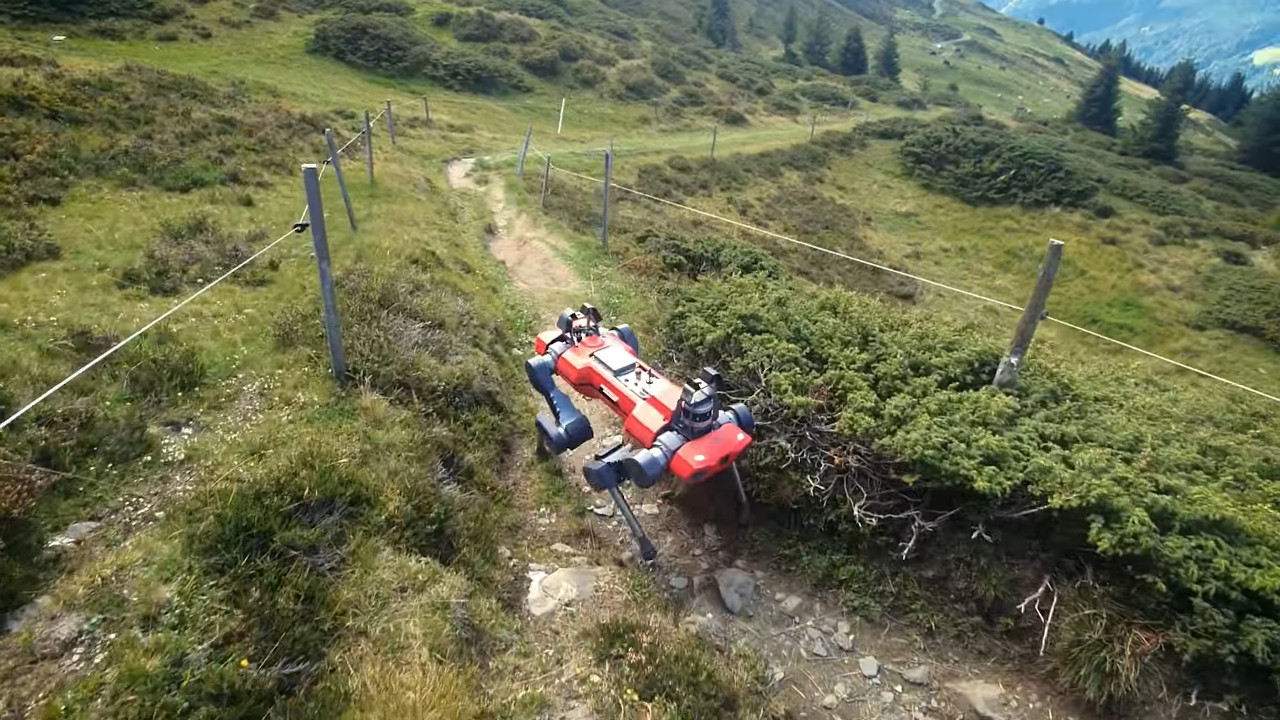
\includegraphics[height=5cm]{figures/hike-with-anymal.jpg}
    \end{figure}
    \begin{center}
        Teacher-student residual reinforcement learning~\cite{lee2020}
    \end{center}
    \blfootnote{Video: \url{https://youtu.be/oPNkeoGMvAE}}
\end{frame}

\begin{frame}{2018: In-hand reorientation}
    \vspace{1.5em}
    \begin{figure}
        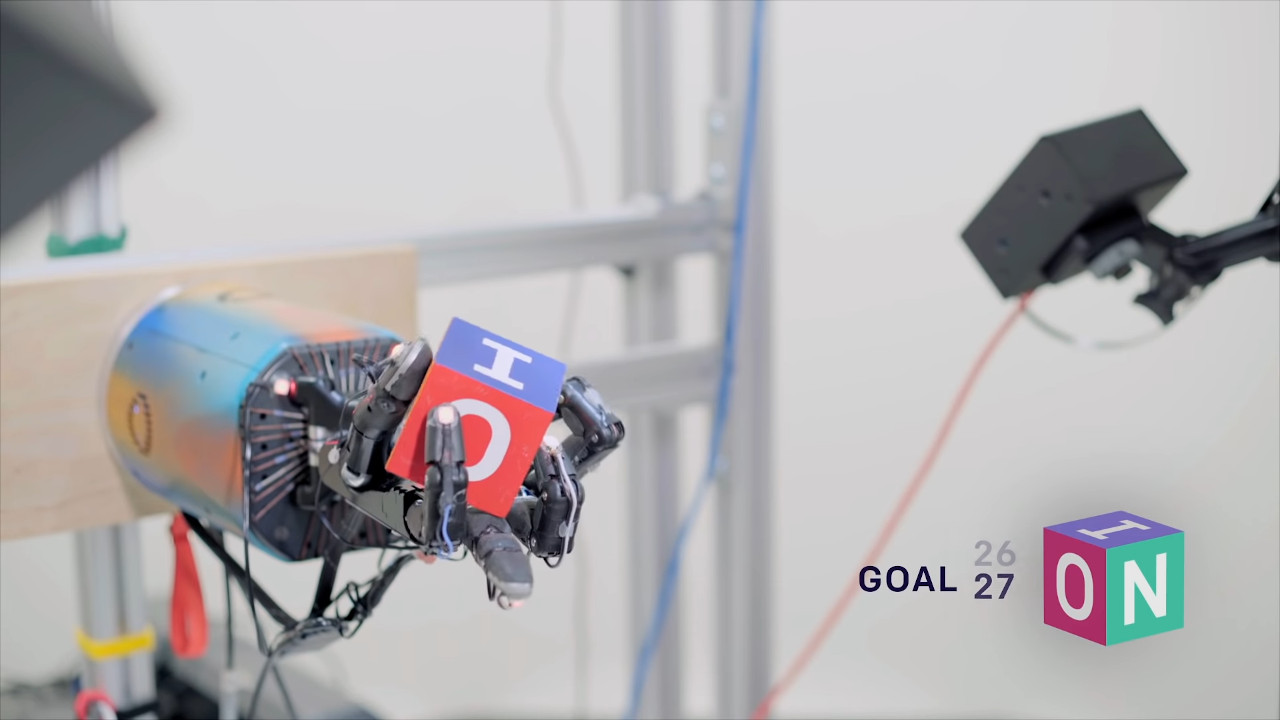
\includegraphics[height=5cm]{figures/in-hand-reorientation.jpg}
    \end{figure}
    \begin{center}
        LSTM policy with domain randomization~\cite{andrychowicz2020learning}
    \end{center}
    \blfootnote{Video: \url{https://youtu.be/jwSbzNHGflM}}
\end{frame}

\begin{frame}{2010: Helicopter stunts}
    \vspace{1.5em}
    \begin{figure}
        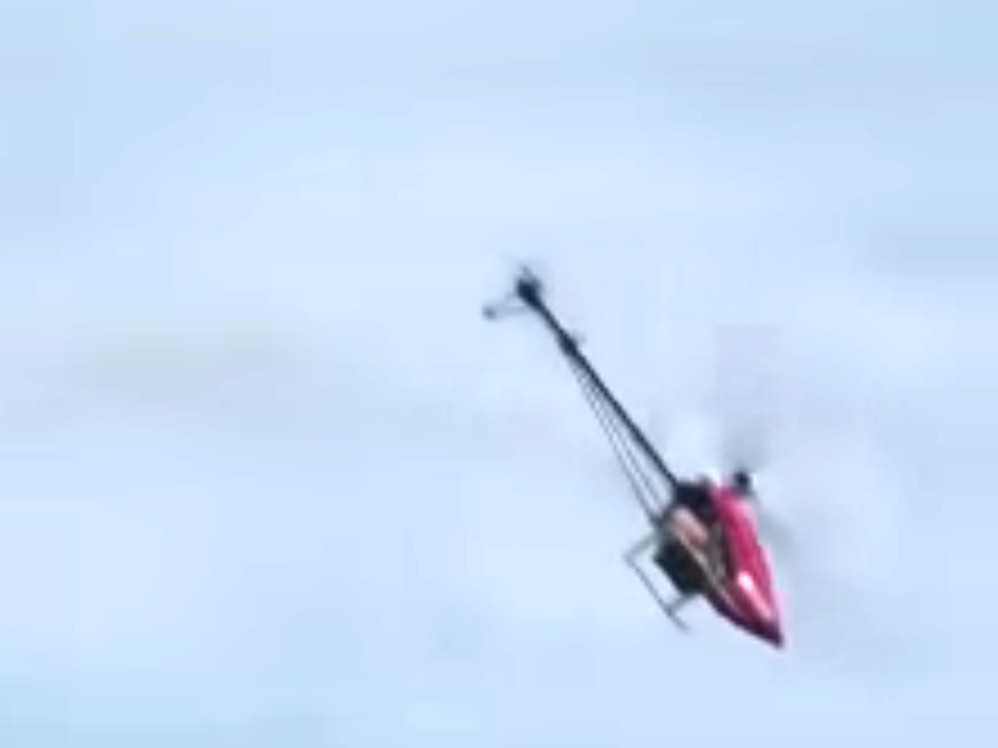
\includegraphics[height=3.5cm]{figures/helicopter-stunts.jpg}
    \end{figure}
    \begin{center}
        Helicopter aerobatics through apprenticeship learning~\cite{abbeel2010}
    \end{center}
    \blfootnote{Video: \url{https://youtu.be/M-QUkgk3HyE}}
\end{frame}

\begin{frame}{1997: Pendulum swing up}
    \vspace{1.5em}
    \begin{figure}
        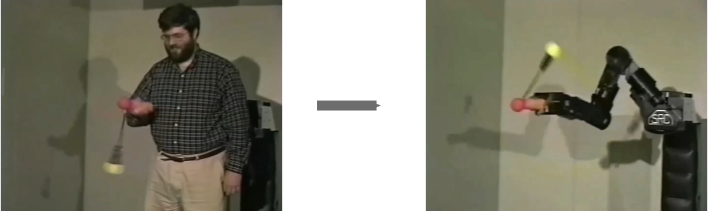
\includegraphics[height=3.5cm]{genfig/atkeson-demo.pdf}
    \end{figure}
    \begin{center}
        Swinging up an inverted pendulum from human demonstrations~\cite{atkeson1997}
    \end{center}
    \blfootnote{ Video: \url{https://youtu.be/g3I2VjeSQUM?t=294} }
\end{frame}

%%%%%%%%%%%%%%%%%%%%%%%%%%%%%%%%%%%%%%%%%%%%%%%%%%%%%%%%%%%%%%%%%%%%%%%%%%%%%%%%

\section*{Basics of reinforcement learning}

\begin{frame}{Scope}
    \begin{figure}
        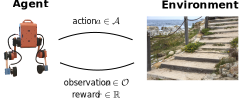
\includegraphics[height=4.5cm]{genfig/agent-environment.pdf}
    \end{figure}
\end{frame}

\begin{frame}{Rewards}
    \begin{figure}
        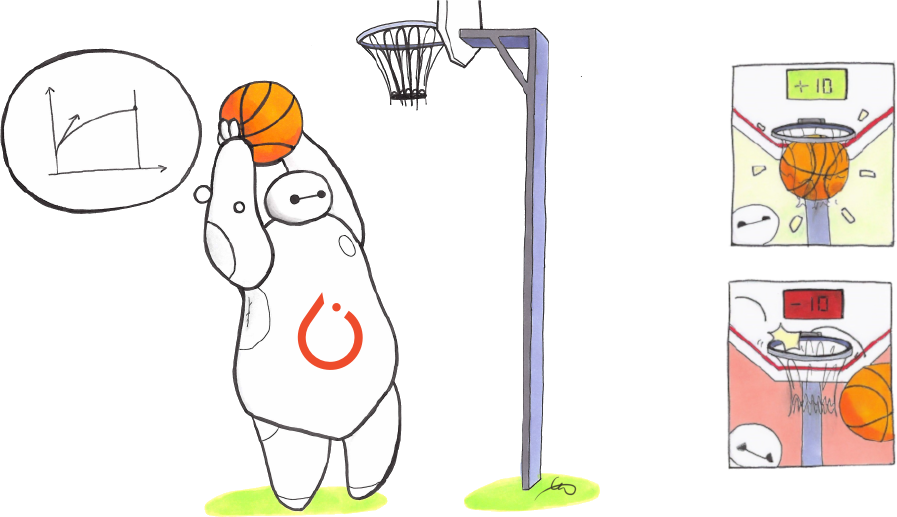
\includegraphics[height=5cm]{figures/stable-baselines3-logo.png}
    \end{figure}
    \blfootnote{
        Image credit: L. M. Tenkes, source: \url{https://araffin.github.io/post/sb3/}
    }
\end{frame}

\begin{frame}{Partially observable Markov decision process (1/2)}
    \begin{figure}
        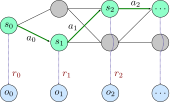
\includegraphics[height=3.5cm]{genfig/pomdp1.pdf}
    \end{figure}
    \begin{itemize}
        \item \textbf{State:} $s_t$, ground truth of the environment
        \item \textbf{Action:} $a_t$, decision of the agent (discrete or continuous)
        \item \textbf{Observation:} $o_t$, \emph{partial} estimation of the state from sensors
        \item \textbf{Reward:} $r_t \in \mathbb{R}$, scalar feedback, often $r_t = r(s_t, a_t)$ or $r(s_t, a_t, s_{t+1})$
    \end{itemize}
    \vspace{-1em}
\end{frame}

\begin{frame}{Partially observable Markov decision process (2/2)}
    \begin{figure}
        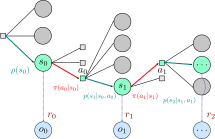
\includegraphics[height=4.5cm]{genfig/pomdp2.pdf}
    \end{figure}
    \begin{table}
        \begin{tabular}{rlll}
            & \emph{Deterministic} & \emph{Stochastic} \\
            \hline
            \textbf{Model:} & $s_{t+1} = f(s_t, a_t)$ & $s_{t+1} \sim p(\cdot | s_t, a_t)$ & how the environment evolves \\
            \textbf{Initial state:} & $s_0$ & $s_0 \sim \rho_0(\cdot)$ & where we start from \\
            \textbf{Observation:} & $o_t = h(s_t)$ & $o_t \sim z(\cdot | s_t)$ & how sensors measure the world \\  % brain cycle
            \textbf{Policy:} & $a_t = g(s_t)$ & $a_t \sim \pi(\cdot | o_t)$ & what the agent decides
        \end{tabular}
    \end{table}
\end{frame}

\begin{frame}[fragile]{Example: The Gymnasium API}
    \begin{figure}
        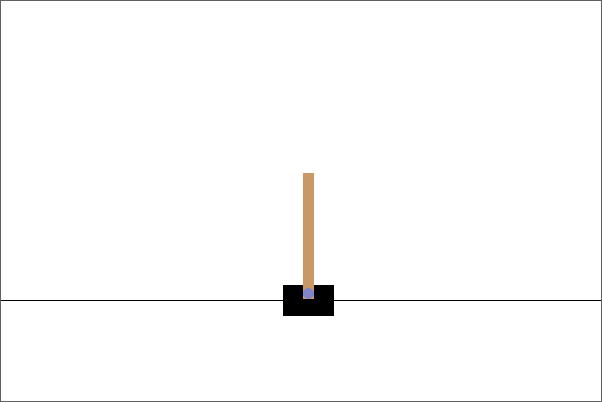
\includegraphics[height=2.5cm]{figures/cart-pole.png}
    \end{figure}
    \begin{minted}{python}
        import gymnasium as gym

        with gym.make("CartPole-v1", render_mode="human") as env:
            env.reset()
            action = env.action_space.sample()
            for step in range(1_000_000):
                observation, reward, terminated, truncated, _ = env.step(action)
                if terminated or truncated:
                    observation, _ = env.reset()
                cart_position = observation[0]
                action = 0 if cart_position > 0.0 else 1
    \end{minted}
\end{frame}

\begin{frame}[fragile]{Same API for simulation and real robots}
    \begin{figure}
        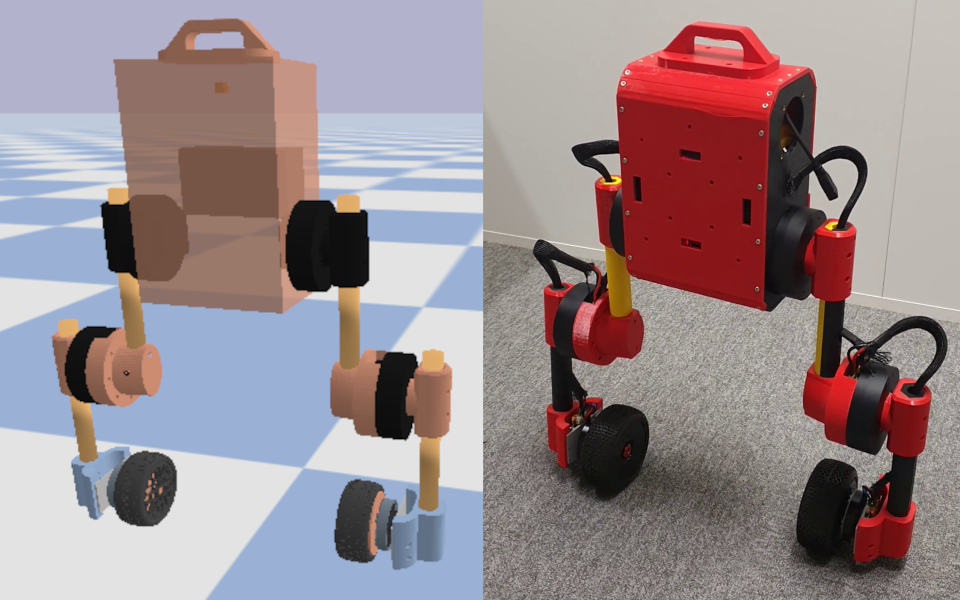
\includegraphics[height=2.5cm]{figures/upkie-sim-real.png}
    \end{figure}
    \begin{minted}{python}
        import gymnasium as gym

        with gym.make("UpkieGroundVelocity-v1", frequency=200.0) as env:
            env.reset()
            action = env.action_space.sample()
            for step in range(1_000_000):
                observation, reward, terminated, truncated, _ = env.step(action)
                if terminated or truncated:
                    observation, _ = env.reset()
                pitch = observation[0]
                action[0] = 10.0 * pitch  # action is [ground_velocity]
    \end{minted}
\end{frame}

\begin{frame}{Goal of reinforcement learning}
    Two last missing pieces:
    \begin{itemize}
        \item \textbf{Episode:} $\tau = (s_0, a_0, r_0, s_1, a_1, r_1, \ldots)$ truncated or infinite\footnote{In practice episodes contain $o_t$ rather than $s_t$. In RL, we implicitly assume that observations contain enough information to be in bijection with their corresponding states. See also \emph{Augmenting observations} thereafter.}
        \item \textbf{Return:} $R(\tau) = \sum_{t \in \tau} r_t$ or with discount $\gamma \in ]0, 1[$: $R(\tau) = \sum_{t \in \tau} \gamma^t r_t$
    \end{itemize}
    We can now state what reinforcement learning is about:

    \vspace{1ex}
    \begin{block}{Goal of reinforcement learning}
        The goal of reinforcement learning is to \emph{find a policy that maximizes returns}.
    \end{block}
\end{frame}

\begin{frame}{Stochastic reinforcement learning}
    In the stochastic setting, the goal of reinforcement learning is:
    \begin{align*}
        \max_{\pi} \ & \mathbb{E}_{\tau} [R(\tau)] \\
        \mathrm{s.t.} \ & \tau = (s_0, a_0, s_1, a_1, \ldots) \\
        & s_0 \sim \rho_0(\cdot) \\
        & o_0 \sim z(\cdot | s_0) \\
        & a_0 \sim \pi(\cdot | o_0) \\
        & s_1 \sim p(\cdot | s_0, a_0) \\
        & \vdots
    \end{align*}
\end{frame}

\begin{frame}{Value functions}
    State value functions $V$:
    \begin{itemize}
        \item \textbf{On-policy:} expected return from a given policy: $V^\pi(s) = \mathbb{E}_{\tau \sim \pi}(R(\tau) | s_0 = s)$
        \item \textbf{Optimal:} best return we can expect from a state: $V^*(s) = \max_\pi \mathbb{E}_{\tau \sim \pi}(R(\tau) | s_0 = s)$
    \end{itemize}
    State-action value functions $Q$:
    \begin{itemize}
        \item \textbf{On-policy:} expected return from following policy: $Q^\pi(s, a) = \mathbb{E}_{\tau \sim \pi}(R(\tau) | s_0 = s, a_0 = a)$
        \item \textbf{Optimal:} best return we can expect: $Q^*(s, a) = \max_\pi \mathbb{E}_{\tau \sim \pi}(R(\tau) | s_0 = s, a_0 = a)$
    \end{itemize}
\end{frame}

\begin{frame}{Components of an RL algorithm}
    A reinforcement-learning algorithm may include any of the following:
    \begin{itemize}
        \item \textbf{Policy:} function approximator for the agent's behavior
        \item \textbf{Value function:} function approximator for the value of states
        \item \textbf{Model:} representation of the environment
    \end{itemize}
    An algorithm with a policy (actor) and a value function (critic) is called \emph{actor-critic}.

    An algorithm with an explicit model is called \emph{model-based} (without: \emph{model-free}).
\end{frame}

\begin{frame}{A taxonomy of RL algorithms}
    \begin{figure}
        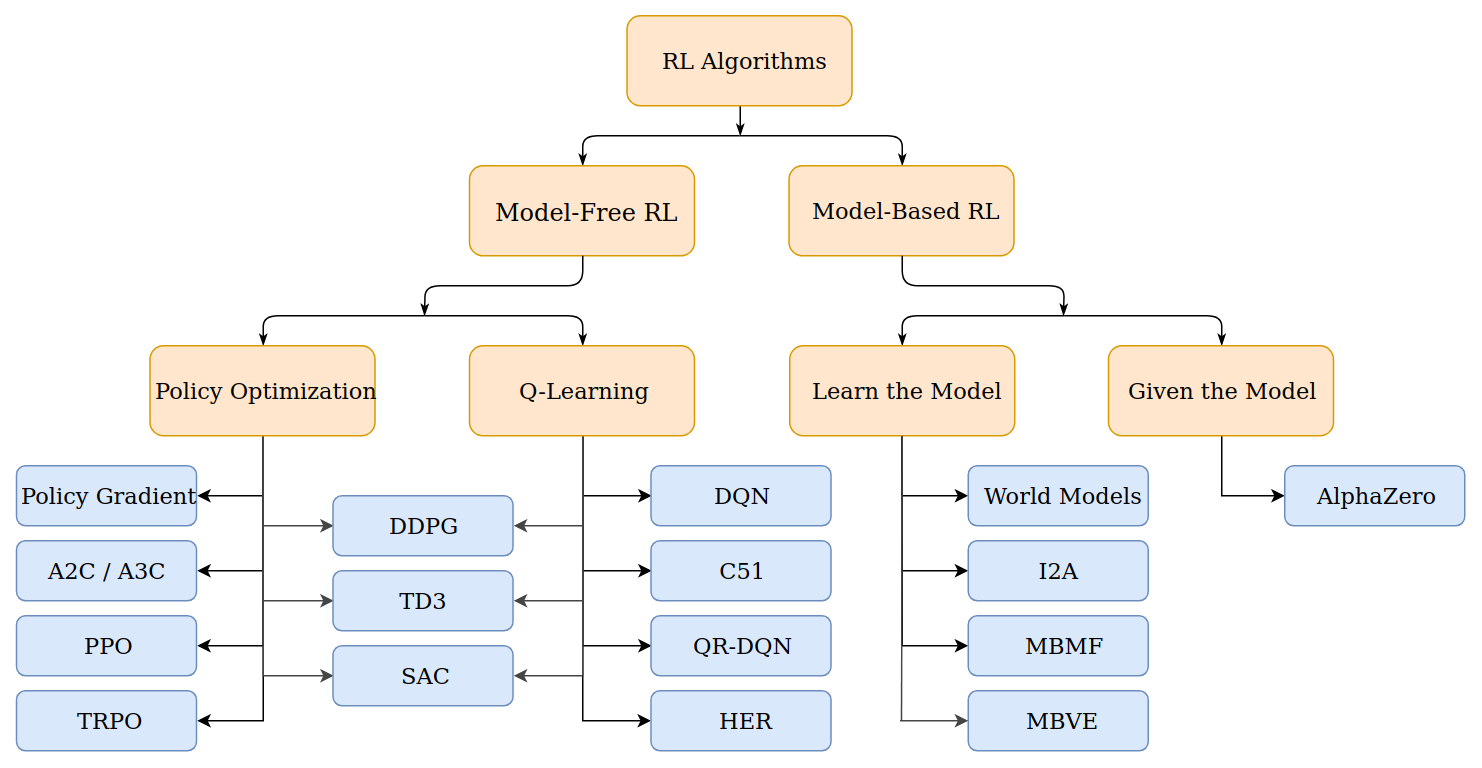
\includegraphics[height=6cm]{figures/taxonomy.png}
    \end{figure}
    \blfootnote{
        There are several taxonomies, none of them fully works. This one is from~\cite{spinningup}.
    }
\end{frame}

\begin{frame}{A taxonomy of RL algorithms}
    \begin{figure}
        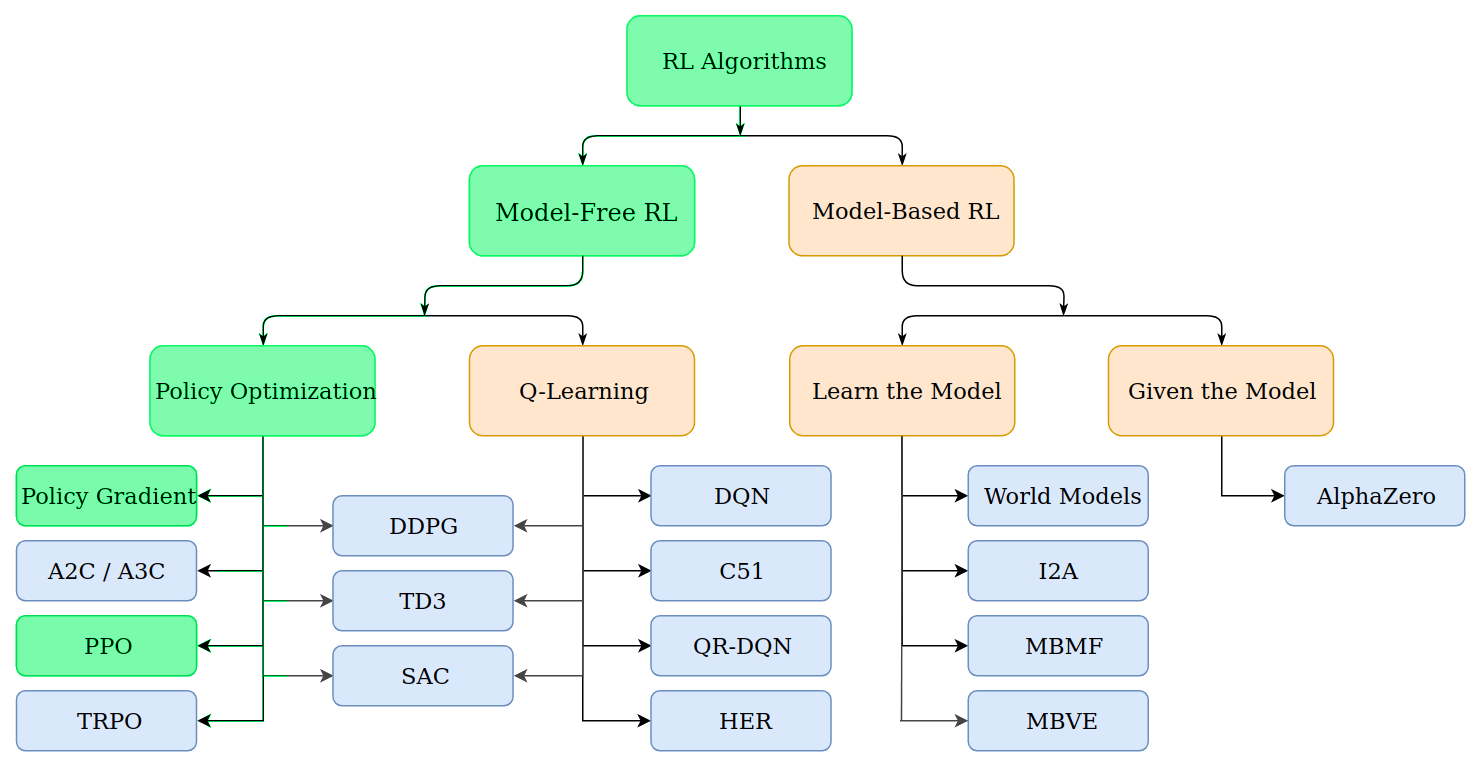
\includegraphics[height=6cm]{figures/taxonomy-focus.png}
    \end{figure}
    \blfootnote{
        Our focus in what follows.
    }
\end{frame}

\section{Policy optimization}

\begin{frame}{Parameterized policy}
    We parameterize our policy $\pi_\theta$ by a vector $\theta \in \mathbb{R}^n$.

    For continuous actions, it is common to use a \emph{diagonal Gaussian policy}:
    \[
        a \sim \pi_\theta(\cdot|s) \ \Longleftrightarrow \ a = \mu_\theta(s) + \mathrm{diag}(\sigma_\theta(s)) z, \ z \sim \mathcal{N}(0, I_m)
    \]
    where $\mu_\theta$ and $\sigma_\theta$ are neural networks mapping states to means and standard deviations.\footnote{In practice, $\sigma$ often does not depend on $s$, and we store $\log \sigma \in \mathbb{R}^m$ rather than $\sigma \in \mathbb{R}^m_+$ in $\theta$.}
\end{frame}

\begin{frame}{Policy-based algorithms}
    A policy-based algorithm updates policy parameters $\theta$ iteratively.

    At each iteration $k$:
    \begin{itemize}
        \item Collect a \emph{batch} of episodes $\mathcal{D}_k = \{ \tau \}$
        \item Apply some update $\theta_{k+1} = \mathit{update}(\theta_k, \mathcal{D}_k)$ to get a new policy $\pi_{\theta_{k+1}}$
    \end{itemize}
\end{frame}

\begin{frame}{Policy optimization}
    The goal of RL is to find a policy that maximizes the expected return. In terms of $\theta$:
    $$
    J(\theta) = \mathbb{E}_{\tau \sim \pi_\theta}[R(\tau)]
    $$
    In policy optimization, we seek an optimum by gradient ascent:
    $$
    \theta_{k+1} = \theta_k + \alpha \nabla_\theta J(\theta_k)
    $$
    The gradient $\nabla_\theta J$ with respect to policy parameters $\theta$ is called the \emph{policy gradient}.
\end{frame}

\begin{frame}{Policy gradient theorem}
    \begin{block}{Policy gradient theorem}
        The policy gradient can be computed from returns and the log-policy gradient $\nabla_\theta \log \pi_\theta$ as:
        \begin{equation*}
            \nabla_\theta J(\theta) = \mathbb{E}_{\tau \sim \pi_\theta} \left(
            R(\tau)
            \sum_{s_t, a_t \in \tau} \nabla_\theta \log \pi_\theta(a_t | s_t)
            \right)
        \end{equation*}
    \end{block}
    LHS: the graal. RHS: things we observe ($R(\tau)$) or know by design ($\nabla_\theta \log \pi_\theta$).
\end{frame}

\begin{frame}{Log-policy gradient example}
    With a diagonal Gaussian policy:
    \begin{align*}
        \log \pi_\theta(a|s) & = -\frac{1}{2} \left[\sum_{i=1}^k \left(\frac{(a_i - \mu_i)^2}{\sigma_i^2} + 2 \log \sigma_i\right) + k \log 2\pi\right] \\
        \nabla_\theta \log \pi_\theta(a|s) & = -\frac{1}{2} \left[ ... \right]
    \end{align*}
\end{frame}

\begin{frame}{Policy gradient theorem: proof sketch}
    \begin{align*}
        \nabla_{\theta} J(\theta)
        & = \nabla_{\theta} \mathbb{E}_{\tau \sim \pi_{\theta}}(R(\tau)) & \text{definition} \\
        & = \nabla_{\theta} \int_{\tau} R(\tau) \mathbb{P}(\tau|\theta) \mathrm{d}\tau & \text{expectation as integral} \\
        & = \int_{\tau} R(\tau) \nabla_{\theta} \mathbb{P}(\tau|\theta) \mathrm{d}\tau & \text{Leibniz integral rule} \\
        & = \int_{\tau} R(\tau) \mathbb{P}(\tau|\theta) \nabla_{\theta} \log \mathbb{P}(\tau|\theta) \mathrm{d}\tau & \text{log-derivative trick} \\
        & = \int_{\tau} R(\tau) \sum_{s_t, a_t \in \tau} \nabla_\theta \log \pi_\theta(a_t | s_t) \mathbb{P}(\tau|\theta) \mathrm{d}\tau & \text{expand $\mathbb{P}(\tau|\theta)$ as product} \\
        & = \mathbb{E}_{\tau \sim \pi_{\theta}} \left(R(\tau) \sum_{s_t, a_t \in \tau} \nabla_\theta \log \pi_\theta(a_t | s_t)\right) & \text{integral as expectation}
    \end{align*}
\end{frame}

\begin{frame}{REINFORCE (1/2)}
    \begin{block}{REINFORCE algorithm~\cite{sutton2018}}
        \centering
        \scalebox{0.8}{
            \begin{algorithm}[H]
                \KwData{initial policy parameters $\theta_0$, learning rate $\alpha$}
                Initialize policy parameters $\theta$ (e.g. to $0$)\;
                \For{$k = 0, 1, 2, \ldots$}{
                    Roll out an episode $\tau = (o_0, a_0, \ldots, o_{N}, a_{N})$ following $\pi_{\theta_k}$\;
                    \For{each step $t \in \tau$}{
                        $R \leftarrow \sum_{t' = t + 1}^N \gamma^{t' - t - 1} r_{t'}$\;
                        $\theta \leftarrow \theta + \alpha \gamma^t R \nabla_\theta \log \pi_\theta(a_t | s_t)$
                }
                }
            \end{algorithm}
        }
    \end{block}
\end{frame}

\begin{frame}{REINFORCE (2/2)}
    Gradient ascent:
    $$
    \theta_{k+1} = \theta_k + \alpha \nabla_\theta J(\theta_k)
    $$
    From the policy gradient theorem, this is equivalent to:
    $$
    \theta_{k+1} = \theta_k + \alpha \mathbb{E}_{\tau \sim \pi_\theta} \left(
            R(\tau)
            \sum_{s_t, a_t \in \tau} \nabla_\theta \log \pi_\theta(a_t | s_t)
            \right)
    $$
    REINFORCE drops the expectation:
    $$
    \theta_{k+1} = \theta_k + \alpha R(\tau_k) \sum_{s_t, a_t \in \tau_k} \nabla_\theta \log \pi_\theta(a_t | s_t)
    $$
\end{frame}

\begin{frame}
    \begin{block}{Vanilla policy gradient~\cite{spinningup}}
        \centering
        \scalebox{0.8}{
            \begin{algorithm}[H]
                \KwData{initial policy parameters $\theta_0$, initial value function parameters $\phi_0$, learning rate $\alpha$}
                \For{$k = 0, 1, 2, \ldots$}{
                    Collect episodes $\mathcal{D}_k = \{ \tau_i \}$ by running $\pi_\theta = \pi(\theta_k)$\;
                    Compute returns $\hat{R}_t$ and advantage estimates $\hat{A}_t$ based on $V_{\phi_k}$\;
                    Estimate the policy gradient as $$\hat{g}_k = \frac{1}{|\mathcal{D}_k|} \sum_{\tau \in \mathcal{D}_k} \sum_{t=0}^T \nabla_\theta \log \left.\pi_\theta(a_t | s_t)\right|_{\theta_k} \hat{A}_t$$
                    \hspace{-0.75em} Update policy parameters by \emph{e.g.} gradient ascent, $\theta_{k+1} = \theta_k + \alpha \hat{g}_k$\;
                    Fit value function by regression on mean-square error: $$\phi_{k+1} = \arg \min_\phi \frac{1}{T |\mathcal{D}_k|} \sum_{\tau \in \mathcal{D}_k} \sum_{t=0}^T \left( \hat{R}_t - V_\phi(s_t)\right)^2$$
                }
            \end{algorithm}
        }
    \end{block}
    \vspace{-1.5em}
\end{frame}

\begin{frame}
    \begin{block}{Proximal policy optimization~\cite{schulman2017proximal}}
        \centering
        \scalebox{0.8}{
            \begin{algorithm}[H]
                \KwData{initial policy parameters $\theta_0$, initial value function parameters $\phi_0$}
                \For{$k = 0, 1, 2, \ldots$}{
                    Collect episodes $\mathcal{D}_k = \{ \tau_i \}$ by running $\pi_\theta = \pi(\theta_k)$\;
                    Compute returns $\hat{R}_t$ and advantage estimates $\hat{A}_t$ based on $V_{\phi_k}$\;
                    \textbf{Clipping:} Update policy parameters by maximizing the clipping objective: $$\theta_{k+1} = \arg \max_\theta \frac{1}{|\mathcal{D}_k| T} \sum_{\tau \in \mathcal{D}_k} \sum_{t=0}^T \min\left( \frac{\pi_\theta(a_t | s_t)}{\pi_{\theta_k}(a_t | s_t)} A^{\pi_{\theta_k}}(s_t, a_t), g(\epsilon, A^{\pi_{\theta_k}}(s_t, a_t)) \right) $$
                    where $g(\epsilon, A) = (1 + \epsilon) A$ if $A \geq 0$ else $(1 - \epsilon) A$

                    Fit value function by regression on mean-square error: $$\phi_{k+1} = \arg \min_\phi \frac{1}{T |\mathcal{D}_k|} \sum_{\tau \in \mathcal{D}_k} \sum_{t=0}^T \left(\hat{R}_t - V_\phi(s_t)\right)^2$$
                }
            \end{algorithm}
        }
    \end{block}
    \vspace{-1.5em}
\end{frame}

\section{Training with PPO}

\begin{frame}{Training}
    \begin{figure}
        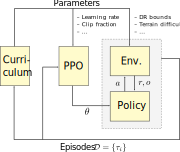
\includegraphics[height=6.5cm]{genfig/training.pdf}
    \end{figure}
\end{frame}

\begin{frame}{Environment}
    \begin{figure}
        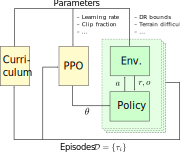
\includegraphics[height=6.5cm]{genfig/training-env.pdf}
    \end{figure}
\end{frame}

\begin{frame}{Rolling out episodes with a simulator}
    \begin{figure}
        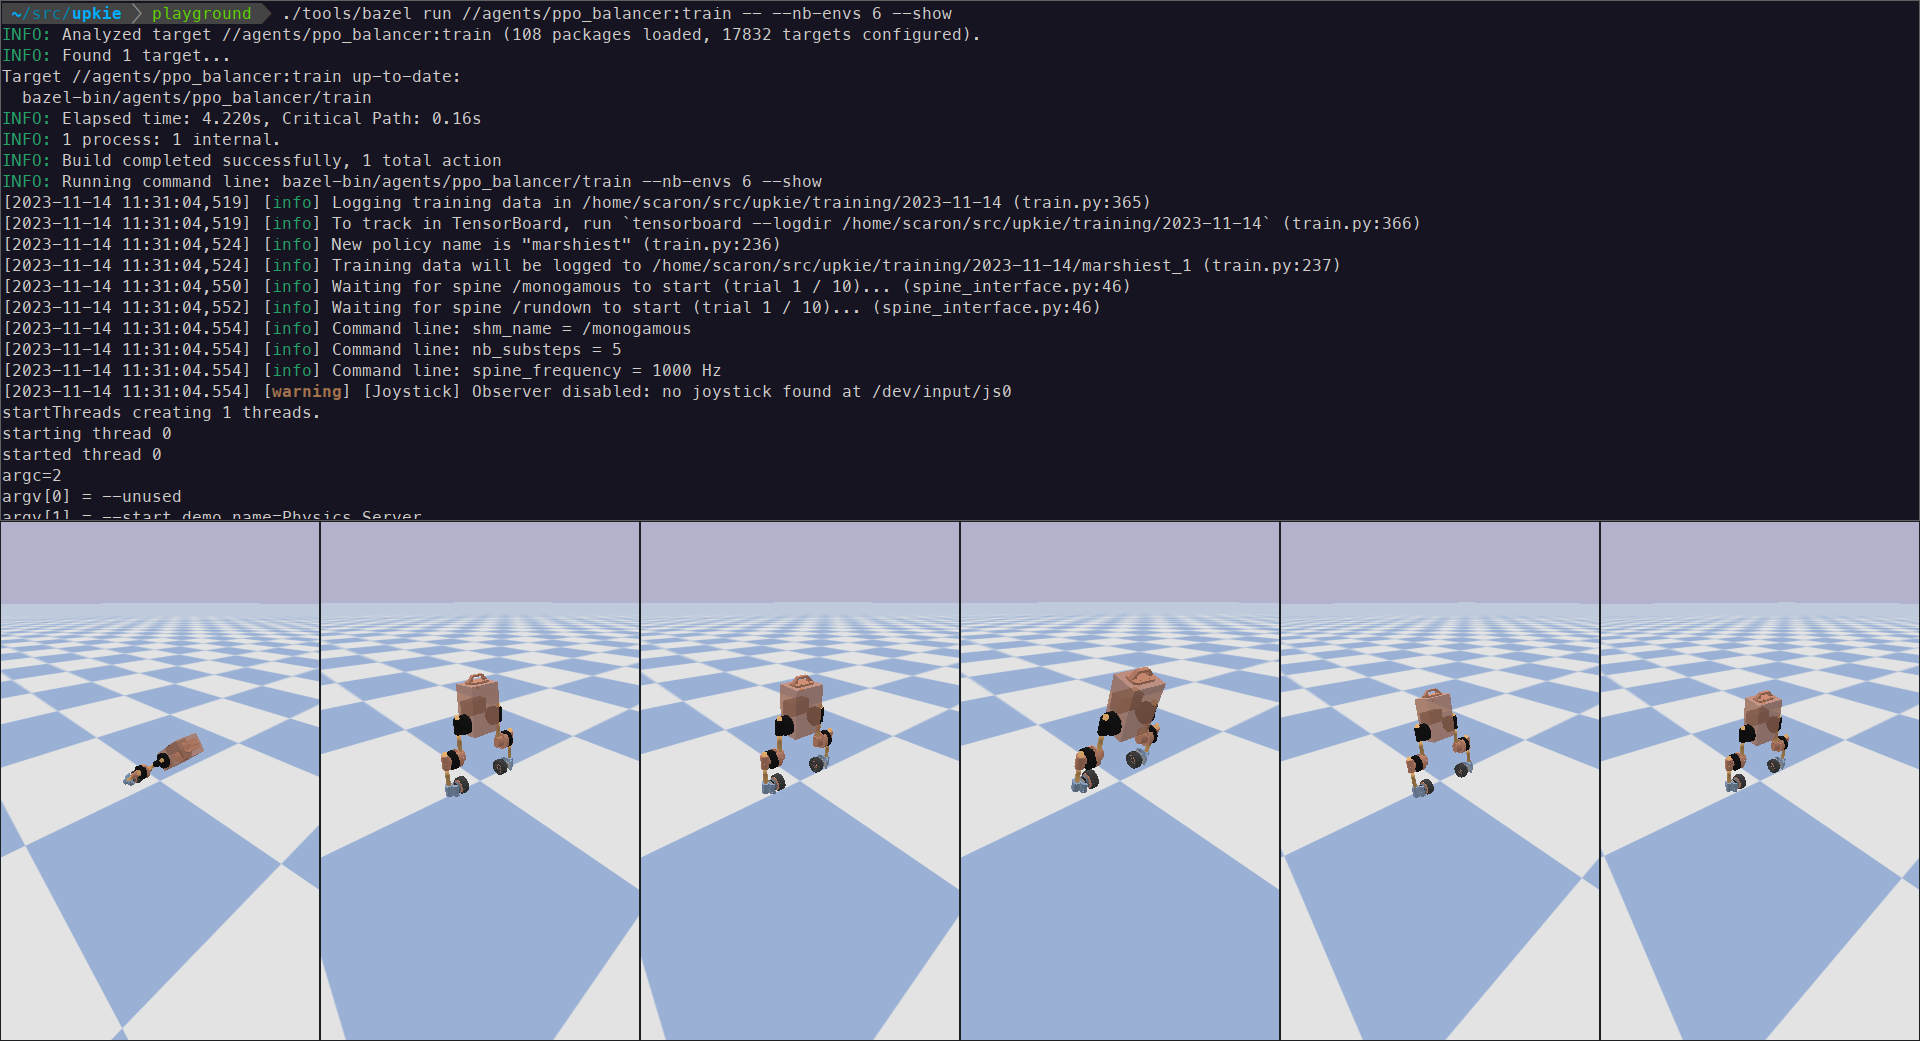
\includegraphics[width=\columnwidth]{figures/upkie-training.png}
    \end{figure}
\end{frame}

\begin{frame}{Curriculum}
    \begin{figure}
        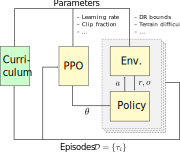
\includegraphics[height=6.5cm]{genfig/training-curriculum.pdf}
    \end{figure}
\end{frame}

\begin{frame}{Monitoring training}
   \begin{adjustbox}{width=\paperwidth, height=\paperheight, keepaspectratio, center}
       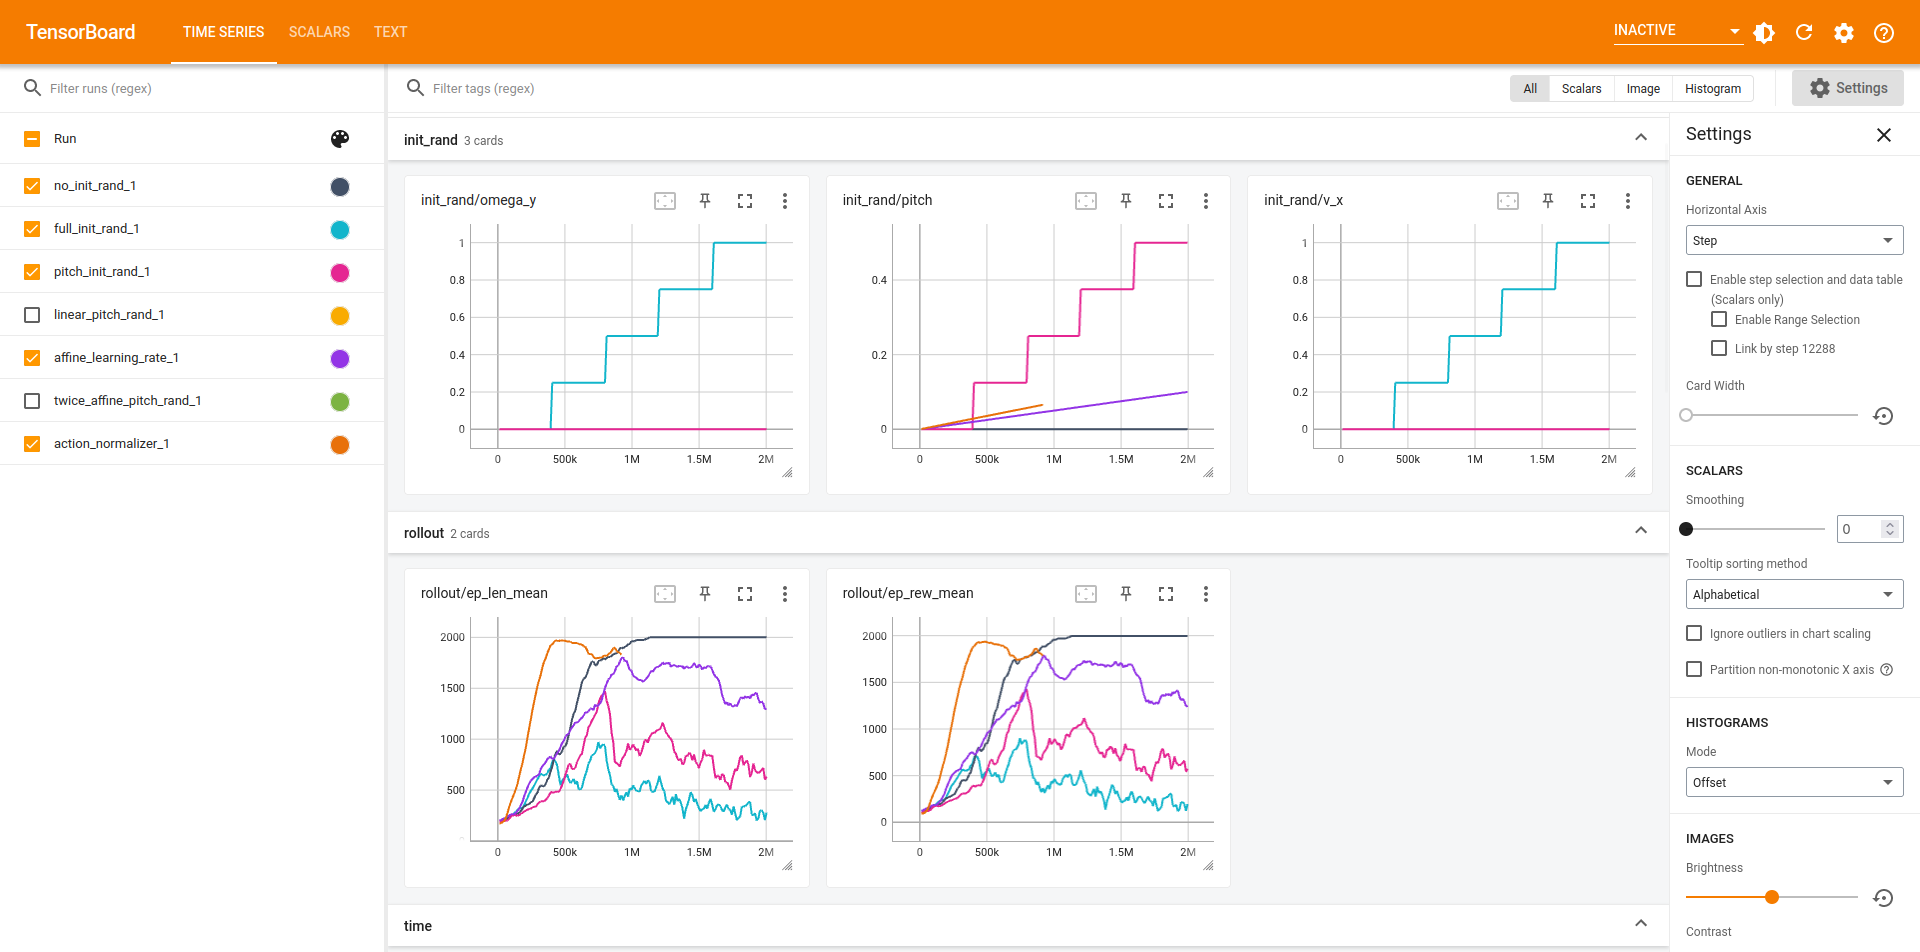
\includegraphics{figures/tensorboard.png}
   \end{adjustbox}
\end{frame}

\begin{frame}{Episode metrics}
    Two main episode metrics:
    \begin{itemize}
        \item \mintinline{python}{ep_len_mean}: average length of an episode, in number of environment steps.
        \item \mintinline{python}{ep_rew_mean}: average return of an episode.
    \end{itemize}
    If training goes well, both eventually plateau at their maximum values.
\end{frame}

\begin{frame}{Training with PPO}
    \begin{figure}
        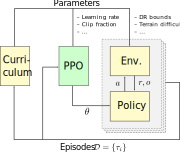
\includegraphics[height=6.5cm]{genfig/training-ppo.pdf}
    \end{figure}
\end{frame}

\begin{frame}{Monitoring PPO}
   \begin{adjustbox}{width=\paperwidth, height=\paperheight, keepaspectratio, center}
        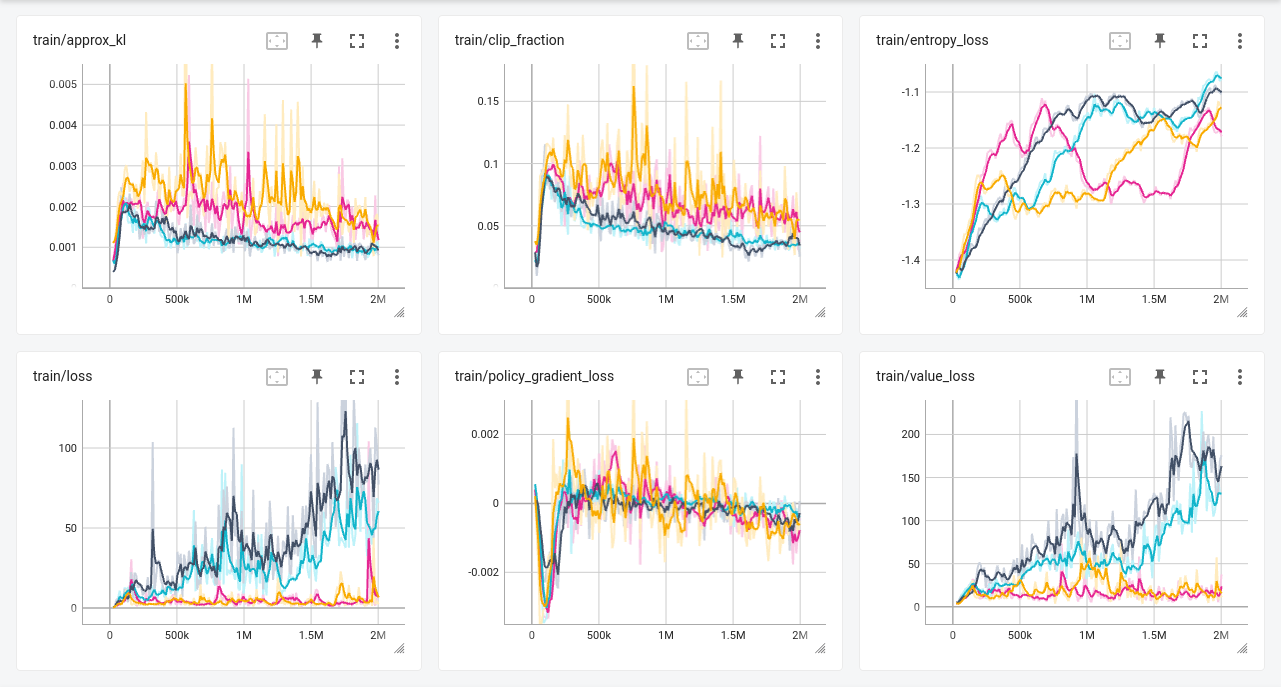
\includegraphics[width=\columnwidth]{figures/tensorboard-ppo.png}
   \end{adjustbox}
\end{frame}

\begin{frame}[fragile]{PPO loss function}
    \begin{block}{Surrogate loss of PPO}
        \mintinline{python}{loss = policy_gradient_loss + ent_coef * entropy_loss + vf_coef * value_loss}
    \end{block}
    \begin{itemize}
        \item \mintinline{python}{policy_gradient_loss}: regular loss resulting from episode returns.
        \item \mintinline{python}{entropy_loss}: negative of the average policy entropy. It should increase to zero over training as the policy becomes more deterministic.
        \item \mintinline{python}{value_loss}: value function estimation loss, \emph{i.e.} error between the output of the function estimator and Monte-Carlo or TD(GAE lambda) estimates.
    \end{itemize}
\end{frame}

\begin{frame}{PPO hyperparameters}
    The PPO implementation in Stable Baselines3 has $> 25$ parameters, including:
    \begin{itemize}
        \item \mintinline{python}{clip_range}: clipping factor in policy loss.
        \item \mintinline{python}{ent_coef}: weight of entropy term in the surrogate loss.
        \item \mintinline{python}{gae_lambda}: parameter of Generalized Advantage Estimation.
        \item \mintinline{python}{net_arch_pi}: policy network architecture.
        \item \mintinline{python}{net_arch_vf}: value network architecture.
        \item \mintinline{python}{normalize_advantage}: use advantage normalization?
        \item \mintinline{python}{vf_coef}: weight of value-function term in the surrogate loss.
    \end{itemize}
\end{frame}

\begin{frame}{Optimizer parameters: steps, epochs, mini-batching}
    The optimizer behind PPO, usually Adam~\cite{kingma2014adam}, comes with parameters:
    \begin{itemize}
        \item \mintinline{python}{learning_rate}: step size parameter, typically decreasing with a linear schedule.
        \item \mintinline{python}{n_steps}: number of environment steps to collect per rollout buffer.
        \item \mintinline{python}{n_epochs}: number of uses of the rollout buffer while optimizing the surrogate loss.
        \item \mintinline{python}{batch_size}: mini-batch size, same as in Stochastic Gradient Descent.
    \end{itemize}
    \begin{figure}
        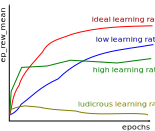
\includegraphics[height=5cm]{genfig/learning-rate.pdf}
    \end{figure}
\end{frame}

\begin{frame}{PPO health metrics}
    Finally, some metrics indicate whether training is going well:
    \begin{itemize}
        \item \mintinline{python}{approx_kl}: approximate KL divergence between the old policy and the new one.
        \item \mintinline{python}{clip_fraction}: mean fraction of policy ratios that were clipped.
        \item \mintinline{python}{clip_range}: value of the clipping factor for the policy ratios.
        \item \mintinline{python}{explained_variance}: $\approx 1$ when the value function is a good predictor for returns.
    \end{itemize}
\end{frame}

\section{Application to robotics}

\begin{frame}{Training a policy}
    General things to do when training a policy:
    \begin{itemize}
        \item Augment observations with history
        \item Observation-action normalization
        \item Curriculum learning
    \end{itemize}
\end{frame}

\begin{frame}{Augmenting observations with history}
    (Welcome to the worst slide of this deck!)
    \begin{itemize}
        \item \textbf{Lag of a system:} number of observations required to estimate its state
        \item We assume the Markov property: $\mathrm{lag} = 1$
        \item Delays in control and physical systems increase their lag
        \item Counter-measure: augment observations with history, restore the Markov property
    \end{itemize}
    RL-trained policies can be remarkable state estimators!
\end{frame}

\begin{frame}{Observation-action normalization}
    Specific to deep RL, normalize the:
    \begin{itemize}
        \item \textbf{Observation space:} bound physical quantities, when possible.
        \item \textbf{Action space:} rescaling to $[-1, 1]$ is common practice.
    \end{itemize}
    Unnormalized actions don't work well on actors with Gaussian outputs (as in PPO):
    \begin{itemize}
        \item Limits too large $\Rightarrow$ sampled actions cluster around zero.
        \item Limits too small $\Rightarrow$ sampled actions saturate all the time, \emph{bang-bang} behavior.
    \end{itemize}
\end{frame}

\begin{frame}{Curriculum learning}
    Domain randomization and task difficulty vary based on policy performance.

    Example: terrain curriculum for quadrupedal locomotion~\cite{lee2020}:
    \begin{figure}
        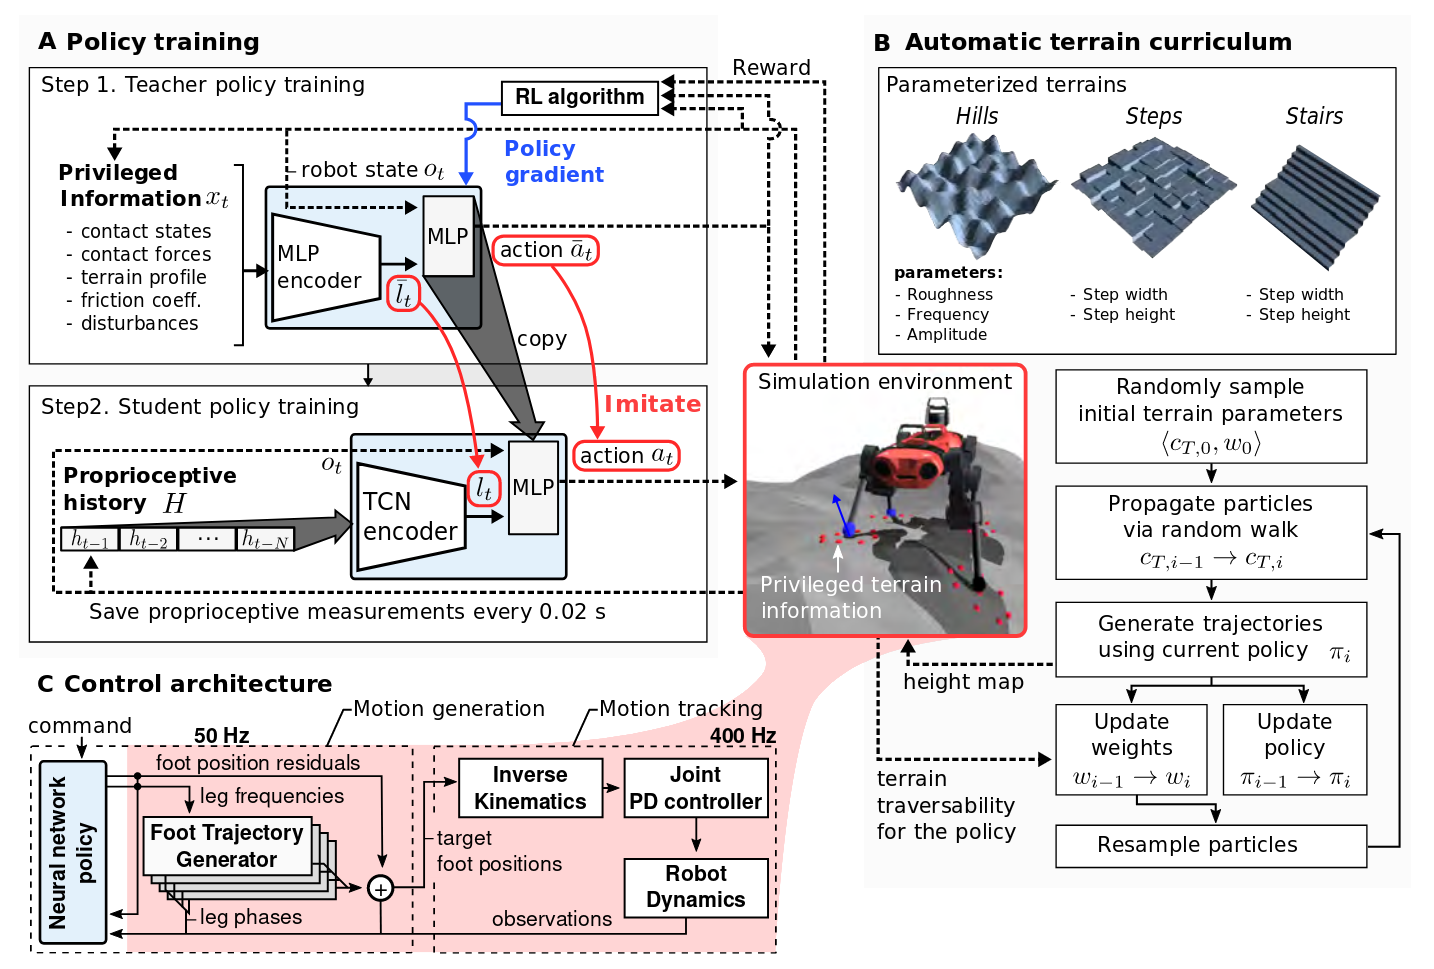
\includegraphics[height=6.7cm]{figures/quadruped-curriculum.png}
    \end{figure}
\end{frame}

\begin{frame}{Sim-to-real gap}
    \begin{figure}
        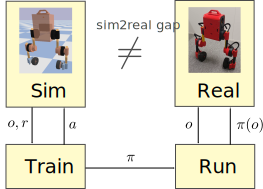
\includegraphics[height=5cm]{genfig/sim2real.pdf}
        \caption{The ``sim-to-real gap'' is a metaphor for model mismatch.}
    \end{figure}
\end{frame}

\begin{frame}{Crossing the sim-to-real gap}
    To improve state observation:
    \begin{itemize}
        \item Teacher-student distillation
    \end{itemize}
    To learn a more robust\footnote{Robustness over model variations.} policy:
    \begin{itemize}
        \item Domain randomization
        \item Data-based simulation
        \item Reward shaping
    \end{itemize}
\end{frame}

% TODO(scaron): distillation
% \begin{frame}{Teacher-student distillation}
%     TODO: Lee et al., RMA, ...
% \end{frame}

\begin{frame}{Domain randomization}
    Randomize selected environment parameters:
    \begin{itemize}
        \item \textbf{Robot geometry:} limb lengths, wheel diameters, \ldots
        \item \textbf{Inertias:} masses, mass distributions
        \item \textbf{Initial state:} $s_0 \sim \rho_0(\cdot)$
        \item \textbf{Actuation models:} delays, bandwidth, \ldots
        \item \textbf{Perturbations:} send $(1 \pm \epsilon) \tau$ torques\ldots
    \end{itemize}
    Domain randomization makes policies more conservative.

    It slows down or completely hampers training.
\end{frame}

\begin{frame}{Data-based actuation models (1/2)}
    \begin{figure}
        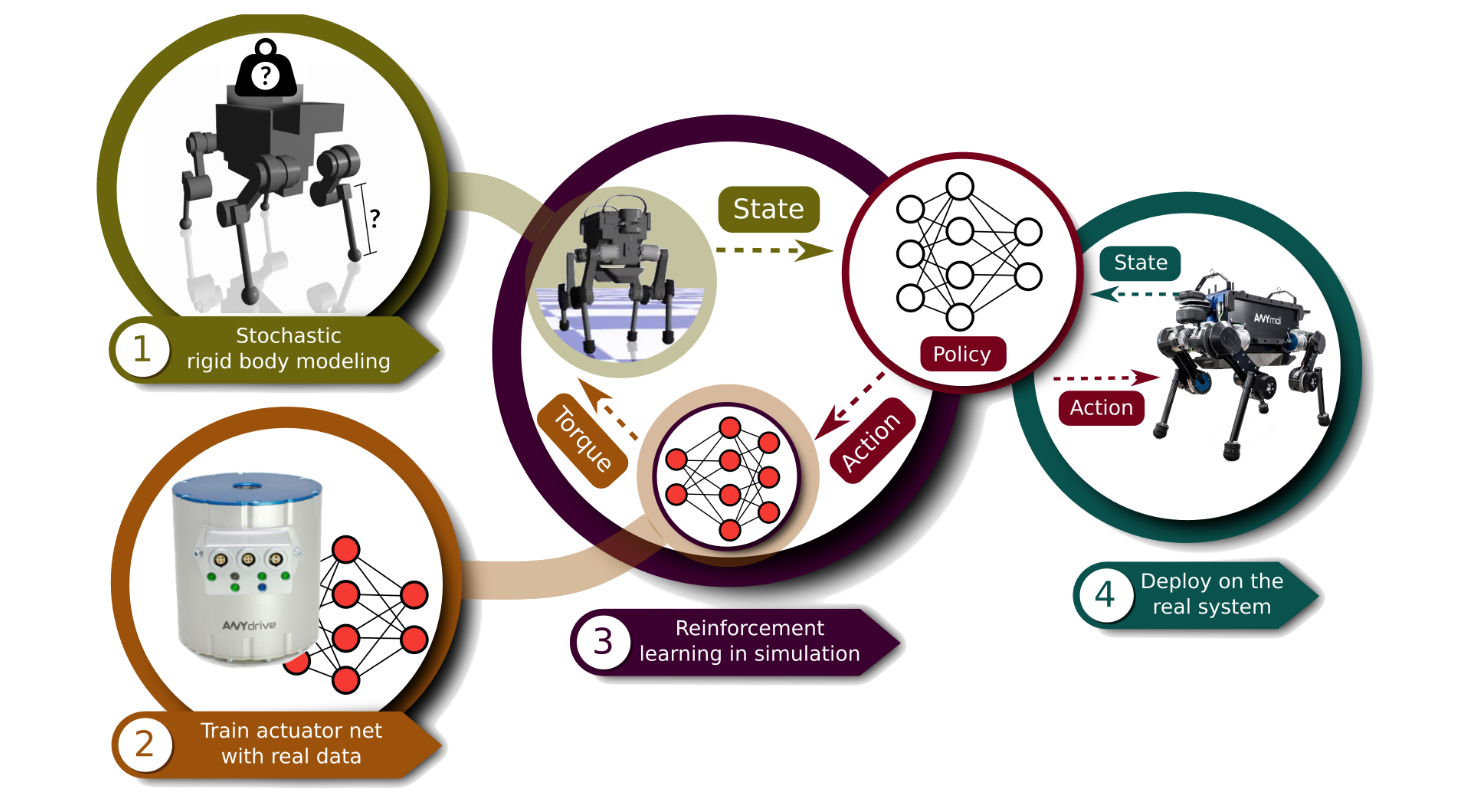
\includegraphics[height=6cm]{figures/quadruped-sim-pipeline.png}
    \end{figure}
    \blfootcite{hwangbo2019}
\end{frame}

\begin{frame}{Data-based actuation models (2/2)}
    \begin{figure}
        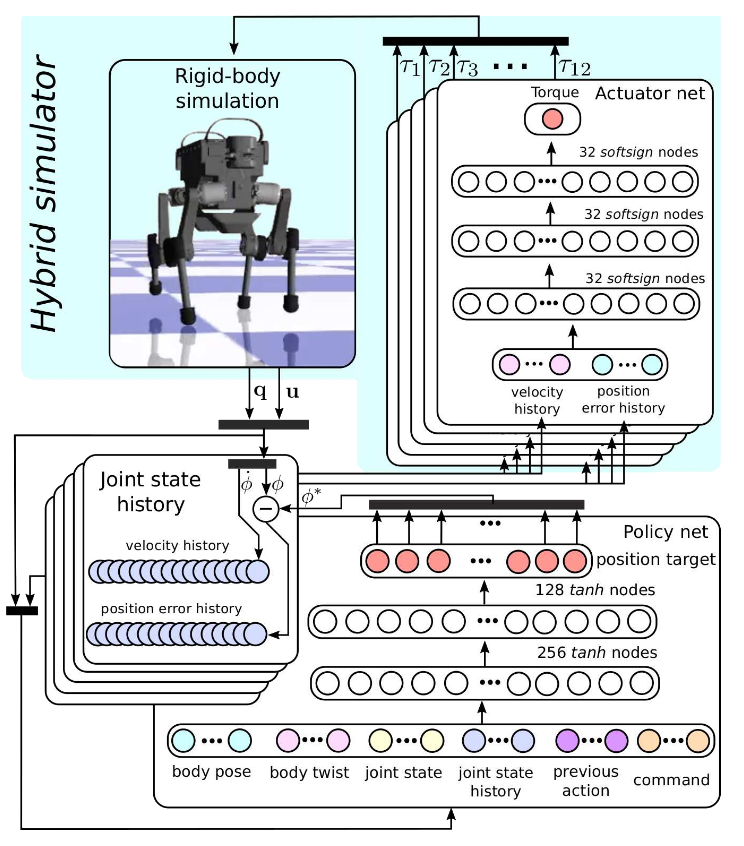
\includegraphics[height=6cm]{figures/quadruped-training.png}
    \end{figure}
    \vspace{-0.7cm}
    \blfootcite{hwangbo2019}
\end{frame}

\begin{frame}{Reward shaping}
    Let $r_e$ denote the reward associated with an error function $e$:

    Motivation:
    \begin{itemize}
        \item Exponential: $r_e = \exp(-e^2)$
    \end{itemize}

    Penalization:
    \begin{itemize}
        \item Absolute value $r_e = -|e|$
        \item Squared value: $r_e = -e^2$
    \end{itemize}
\end{frame}

\begin{frame}{RewArt}
    Making an RL pipeline work can lead to complex rewards, e.g. in~\cite{lee2020}:
    \begin{itemize}
        \item Linear velocity tracking: $r_{lv} = \exp(-2.0 (v_{pr} - 0.6)^2)$, or 1, or 0
        \item Angular velocity tracking: $r_{av} = \exp(-1.5 (\omega_{pr} - 0.6)^2)$, or 1
        \item Base motion tracking: $r_b = \exp(-1.5v_o^2) + \exp(-1.5 \|({}^B_{IB} \omega)_{xy}\|^2)$
        \item Foot clearance: $r_{fc} = \sum_{i \in I_{swing}} \mathbf{1}_{fclear}(i) / |I_{swing}|$
        \item Body-terrain collisions: $r_{bc} = -|I_{c,body} \textbackslash I_{c,foot}|$
        \item Foot acceleration smoothness: $r_{s} = -\| (r_{f,d})_t - 2(r_{f,d})_{t-1} + (r_{f,d})_{t-2}\|$
        \item Torque penalty: $r_{\tau} = -\sum_{i} | \tau_i |$
    \end{itemize}
    Final reward: $r = 0.05 r_{lv} + 0.05 r_{av} + 0.04 r_b + 0.01 r_{fc} + 0.02 r_{bc} + 0.025 r_s + 2 \cdot 10^{-5} r_{\tau}$
\end{frame}

\begin{frame}{Example: Upkie ground velocity}
    \textbf{Observation:}
    \begin{table}
        \begin{tabular}{|l|l|l|}
            \hline
            \textbf{Index} & \textbf{Symbol} & \textbf{Description} \\
            \hline
            0 & $\theta$ & pitch from torso to inertial frame \\
            1 & $p$ & ground position \\
            2 & $\dot{\theta}$ & pitch angular velocity from torso to inertial frame \\
            3 & $\dot{p}$ & ground velocity \\
            \hline
        \end{tabular}
    \end{table}
    \textbf{Action:}
    \begin{table}
        \begin{tabular}{|l|l|l|}
            \hline
            \textbf{Index} & \textbf{Symbol} & \textbf{Description} \\
            \hline
            0 & $v$ & commanded ground velocity \\
            \hline
        \end{tabular}
    \end{table}
\end{frame}

\begin{frame}{Example: Rewards}
    RewArt is not a necessity: advocacy for simple rewards.

    In the Upkie ground-velocity environment, we went for:
    \begin{align*}
        p_{\mathit{tip}} & = p + \ell \sin(\theta) \\
        r(o) & := \exp\left(-\left(\frac{p_{\mathit{tip}}}{\sigma}\right)^2\right)
    \end{align*}
    Including higher-order derivatives does not always help.
\end{frame}

\begin{frame}{Example: environment wrappers}
    Composability of environments helps while prototyping. In the Upkie
    ground-velocity environment:
    \begin{itemize}
        \item Base environment: velocity commands
        \item (Training:) add action noise
        \item (Training:) add observation noise
        \item \textbf{(Training:) low-pass filter on wheel actuators}
        \item \textbf{Include last ten observation-action pairs in observation vector}
        \item Change action to ground acceleration (with bounds)
        \item \textbf{Rescale action between $-1$ and $1$}
    \end{itemize}
\end{frame}

\begin{frame}{Keep in mind that we are in a stochastic world}
    \begin{figure}
        \centering
        \only<1>{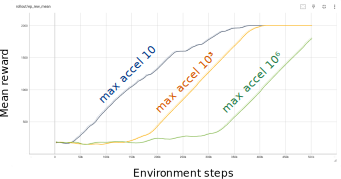
\includegraphics[height=5cm]{genfig/max-accel.pdf}}
        \only<2>{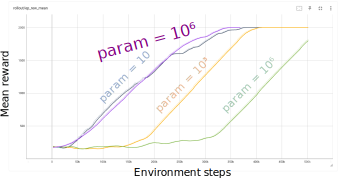
\includegraphics[height=5cm]{genfig/max-accel-bis.pdf}}
        \caption{
            \only<1>{We may be observing the effect of our parameter.}
            \only<2>{Or we may be observing the variance of the training process.}
        }
    \end{figure}
\end{frame}

\begin{frame}{Challenges for RL}
    \begin{itemize}
        \item \textbf{Sim-to-real:} no one-size-fits-all method, depends on robot and task
        \item \textbf{Jittering:} action noise, due to need for stochastic policies (PGT!)
        \item \textbf{Sample efficiency:} requires millions of samples $(s_t, a_t, s_{t+1})$
        \item \textbf{Reward shaping:} often helps, not a necessity, ``RewArt''!
        \item \textbf{Curriculum learning:} humans monitoring computers that learn\footnote{ Also known as SGD: ``Student Grad Descent''}
    \end{itemize}
\end{frame}

\section{What did we see?}

\begin{frame}{What we saw}
    Introduction to policy optimization:
    \begin{itemize}
        \item Partially-observable Markov decision process (POMDP)
        \item The goal of reinforcement learning
        \item Model, policy and value function
        \item Policy optimization: REINFORCE, policy gradient, PPO
    \end{itemize}
    Application to robotics:
    \begin{itemize}
        \item Training policies: add history, normalization, curriculum
        \item Sim-to-real gap: domain randomization, data-based sim, ``RewArt''
    \end{itemize}
    RL is not magic: great results, possibly going to great lengths!
\end{frame}

\begin{frame}[standout]
    Thank you for your attention!\footnote{\color{white} Thanks to Elliot Chane-Sane, Thomas Flayols, Nicolas Perrin-Gilbert, Philippe Sou\`{e}res and the 2023 class at MVA for feedback on previous versions of these slides.}
\end{frame}

\section*{Bibliography}

\renewcommand*{\bibfont}{\footnotesize}
\setbeamertemplate{bibliography item}{\insertbiblabel}
\begin{frame}[allowframebreaks]{References}
    \printbibliography[heading=none]
\end{frame}

\section{Bonus slides}

% \begin{frame}{Link between discount and time window}
%     Context:
%     \begin{itemize}
%         \item One observation-action cycle lasts $\Delta t > 0$
%         \item We focus on the next $T = N \Delta t$ steps, $N \in \mathbb{N}$
%     \end{itemize}
%     Then, taking $\gamma = 1 - \frac{\Delta t}{T}$, ...
% \end{frame}

\begin{frame}{Bellman equation}
    Value functions satisfy the Bellman equation:
    \begin{block}{Bellman equation}
        \[
            V^*(s) = \max_\pi \mathbb{E}_{a \sim \pi(\cdot | s), (r, s') \sim p(s' | s, a)}[r + \gamma V^*(s')]
        \]
    \end{block}
    This is a connection to optimal control (\emph{e.g.} differential dynamic programming) and $Q$-learning, but not our topic today.
\end{frame}

\begin{frame}{Intuition behind clipping in PPO}
    When the advantage is positive:

    $$L(s,a,\theta_k,\theta) = \min\left( \frac{\pi_{\theta}(a|s)}{\pi_{\theta_k}(a|s)}, (1 + \epsilon) \right) A^{\pi_{\theta_k}}(s,a)$$

    The objective increases if the action becomes more likely $\pi_{\theta}(a|s) > \pi_{\theta_k}(a|s)$, but no extra benefit as soon as $ \pi_{\theta}(a|s) > (1+\epsilon) \pi_{\theta_k}(a|s)$.

    When the advantage is negative: \emph{idem} \emph{mutatis mutandis}.
\end{frame}

\end{document}
